\documentclass{article}
\usepackage[final]{neurips_2019}

\usepackage[utf8]{inputenc} % allow utf-8 input
\usepackage[T1]{fontenc}    % use 8-bit T1 fonts
\usepackage{hyperref}       % hyperlinks
\usepackage{url}            % simple URL typesetting
\usepackage{booktabs}       % professional-quality tables
\usepackage{amsfonts}       % blackboard math symbols
\usepackage{nicefrac}       % compact symbols for 1/2, etc.
\usepackage{microtype}      % microtypography
\usepackage{amsmath}
\usepackage{graphicx}
\title{Exeriese 2}

\author{%
  Lan Zhang\\
  954517477\\
}

\begin{document}
\maketitle

\section{Problem 1}

Solved on 09/17/2019. The seed I used for noise generation is 2612.

\subsection{Loss Function}

Given an input $x$ with an output $y$, the prediction is $\hat{y}$. The performance of squared loss function shows in Figure\ref{squared_loss_fuc}. 

The formulation of squared loss is:
$$squared\_loss = \frac{1}{N}\sum_0^N{(y_i - \hat{y_i})^2}$$

Given the parameter delta = 1.0. The formulation of huber loss is:
$$huber\_loss = \left\{\begin{matrix}
0.5 *  (y - \hat{y})          & if |(y - \hat{y})| <= d\\ 
d*|(y - \hat{y})| - 0.5 * d^2 & if |(y - \hat{y})| >  d
\end{matrix}\right.$$

The performance of huber loss function shows in Figure\ref{huber_loss_fuc}. 

I also implement the following hybrid loss function and the performance shows in Figure \ref{hybrid_loss}. 
$$hybrid\_loss = huber\_loss + |y - \hat{y}|$$

If I didn't use $tf.reduce\_mean$ in squared loss, the result of parameters $W$ and $b$ will turn out to be NaN. I found the issue will happen on tensorflow 2.0. But on tensorflow 1.14, sometimes it can output a correct answer. I'm not sure about the reason. but I think it maybe because something lead to overflow at some point during gradient descent and cause NaNs.

It's hard to tell which loss function works better(see Figure\ref{all_loss}). I've run the code with those two loss function multiple times and both of them work well. If I use the distance of the predicted parameters $W, b$ and original parameters$W, b$ as a measure of the performance, the squared loss(.0133321) work better than huber loss(.0238144).

\begin{figure}
  \centering
  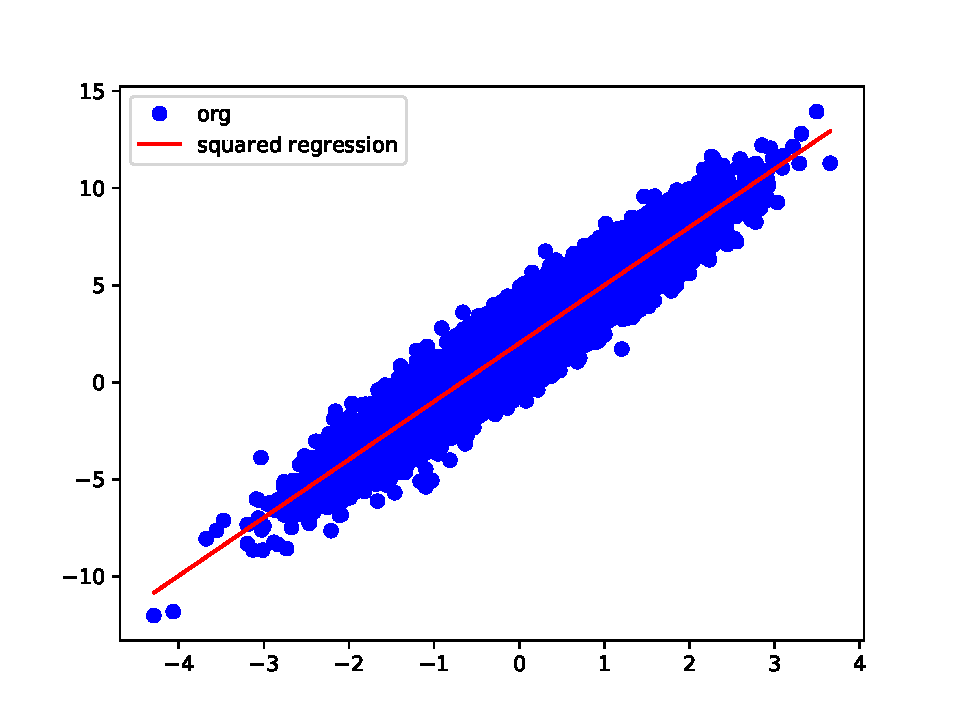
\includegraphics[scale=0.5]{imgs/squared.pdf}
  \caption{Squared loss}
  \label{squared_loss_fuc}
\end{figure}

\begin{figure}
  \centering
  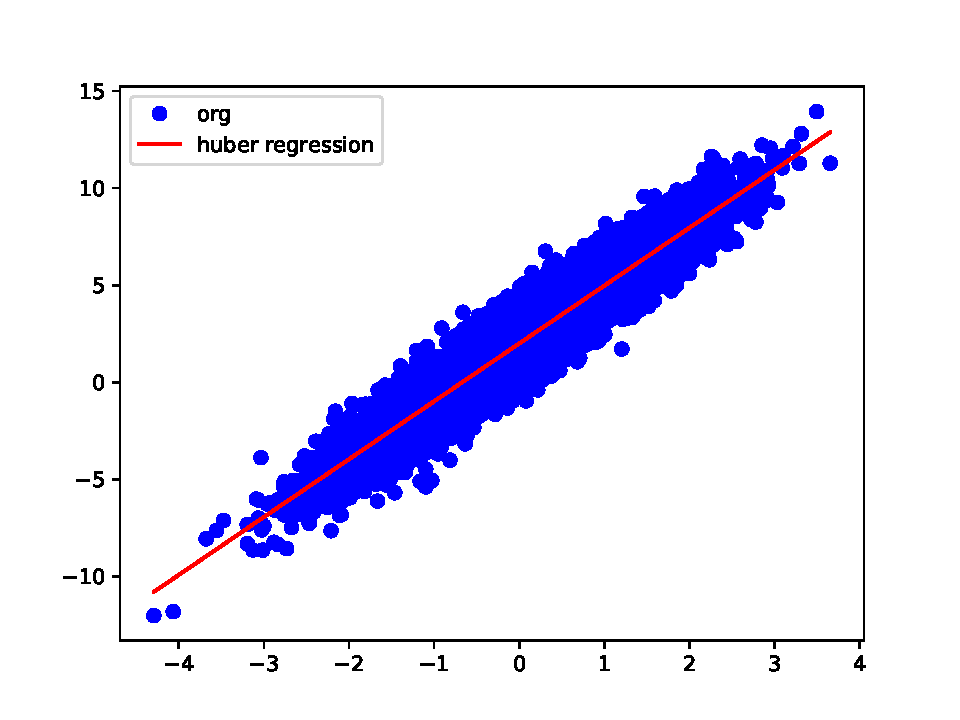
\includegraphics[scale=0.5]{imgs/huber.pdf}
  \caption{Huber loss}
  \label{huber_loss_fuc}
\end{figure}

\begin{figure}
  \centering
  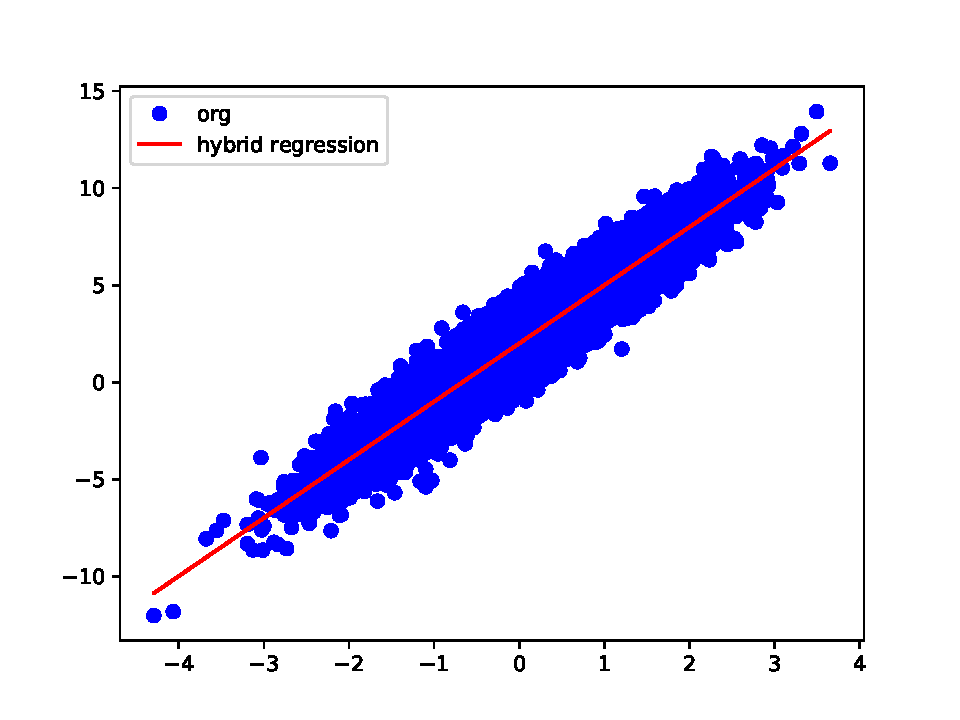
\includegraphics[scale=0.5]{imgs/hybrid.pdf}
  \caption{Hybrid loss}
  \label{hybrid_loss}
\end{figure}

\begin{figure}
  \centering
  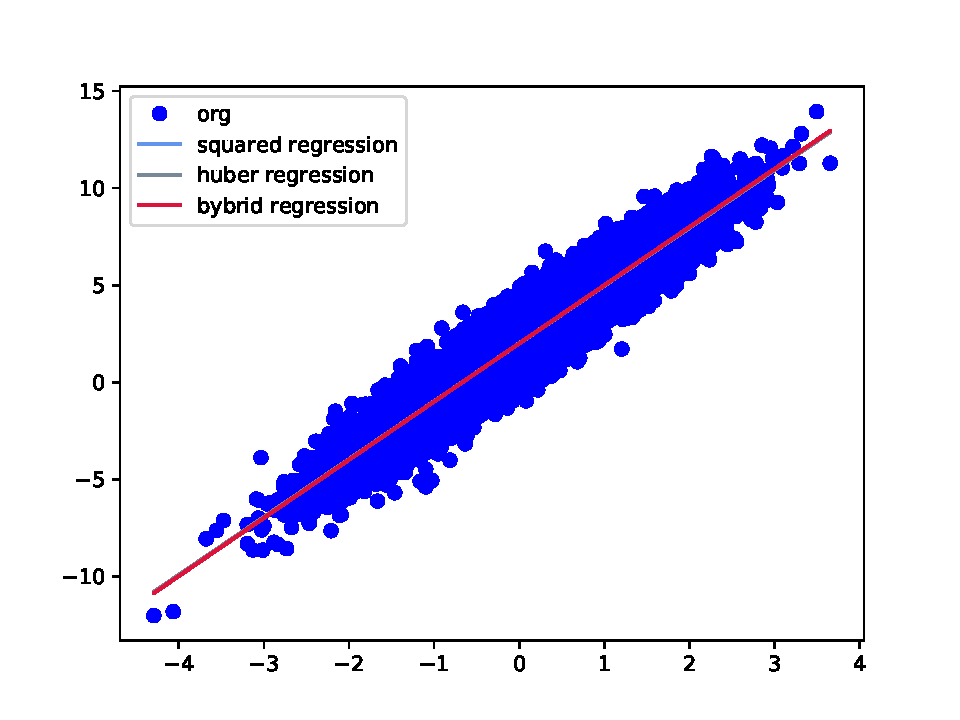
\includegraphics[scale=0.5]{imgs/all.pdf}
  \caption{Performance of different loss}
  \label{all_loss}
\end{figure}


\subsection{Learning rate}

I implemented patience scheduling. Then I tested learning rate from 0.001 to 0.01 with the incrementation 0.002, Shown in Figure \ref{lr}. The result are quite similar. Table \ref{tab:lr} shows the parameters learned under different learning rate with patience scheduling.

\begin{figure}
  \centering
  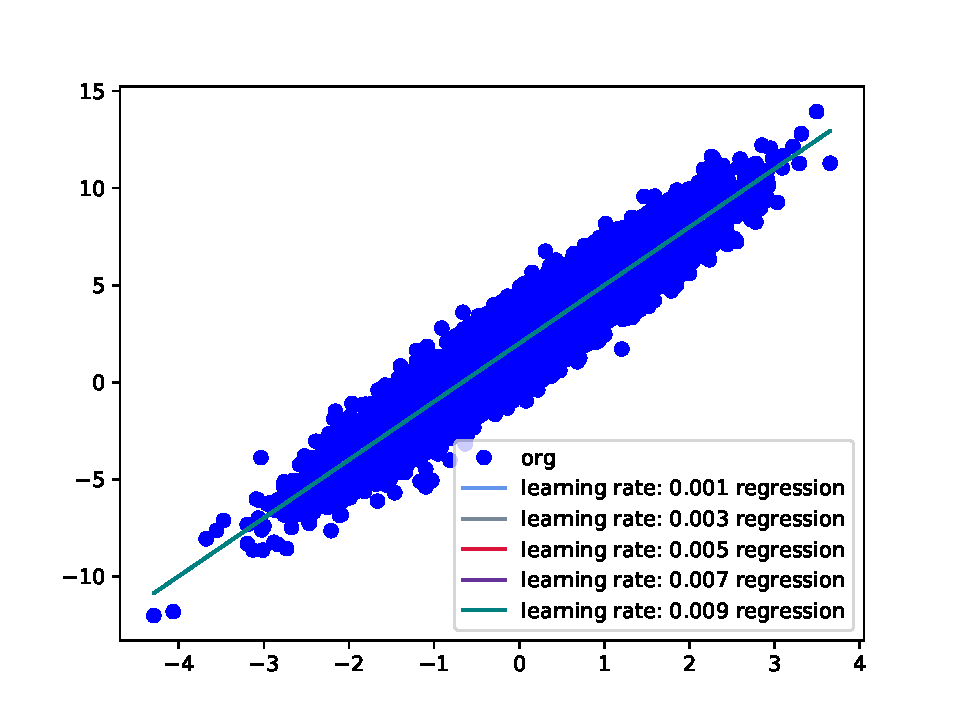
\includegraphics[scale=0.5]{imgs/lr.pdf}
  \caption{Learning rate}
  \label{lr}
\end{figure}

\begin{table}
  \caption{The performance of different learning rate}
  \label{tab:lr}
  \centering
  \begin{tabular}{lll}
    \toprule
    Learning rate     & W     & b \\
    \midrule
    0.001 & 2.9962702  & 2.0017185     \\
    0.003     & 2.9964287 & 2.001716     \\
    0.005     & 2.996503       & 2.0016577  \\
    0.007     & 2.996541 & 2.001543      \\
    0.009     & 2.9966085      & 2.0013998  \\
    \bottomrule
  \end{tabular}
\end{table}

\subsection{Training steps}
I've tested different training steps from 500 to 1500 with the incrementation 200. Shown in Figure \ref{ts}. With longer duration, the performance tend to be better. However, after "enough" steps, this effects start to stabilize and even decrease(see Table \ref{tab:ts}).

\begin{table}
  \caption{The performance of different training steps}
  \label{tab:ts}
  \centering
  \begin{tabular}{lll}
    \toprule
    Training steps     & W     & b \\
    \midrule
    500 & 2.9877446  & 1.9952948     \\
    700     & 2.995941 & 2.001462     \\
    900     & 2.9962356       & 2.0016909  \\
    1100     & 2.9962835 & 2.001727      \\
    1300    & 2.9962983      & 2.0017405  \\
    \bottomrule
  \end{tabular}
\end{table}

\begin{figure}
  \centering
  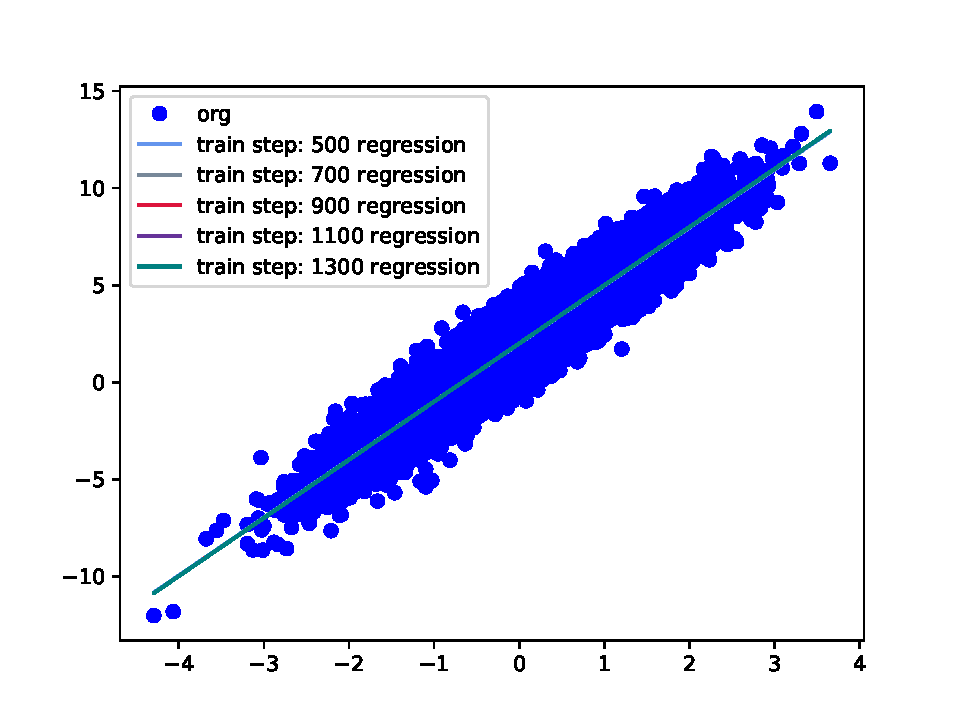
\includegraphics[scale=0.5]{imgs/ts.pdf}
  \caption{Training steps}
  \label{ts}
\end{figure}

\subsection{Initial Value of parameters}
Table \ref{tab:w} and Table \ref{tab:b} respectively denote predicted parameters with different initial parameter W and b(both of them are from -1000 to 1000 with the incrementation 500).

If I initialize the parameter W with a small number like -1000 with hybrid Loss, the predicted parameter W will become -984.0698 after 1000 epochs. That is because the model has not yet converged after 1000 epochs. Figure \ref{epoch} is the performance of different traing epoch with the initial parameter $W=-100$. Desipt the predicted parameters after 9000 epochs are far from the correct answer, it is gradually approaching to the correct answer.

\begin{table}
  \caption{The performance of different W after 1000 epochs}
  \label{tab:w}
  \centering
  \begin{tabular}{lll}
    \toprule
    Initial W     & W     & b  \\
    \midrule
    -1000 & -984.0698 & -0.16686472    \\
    -500     & -484.0088 & -0.12897438     \\
    0     & 2.9962702      & 2.0017185  \\
    500     & 484.0088 & 0.2609221     \\
    1000    & 984.0698     & 0.22580884  \\
    \bottomrule
  \end{tabular}
\end{table}

\begin{table}
  \caption{The performance of different b after 1000 epochs}
  \label{tab:b}
  \centering
  \begin{tabular}{lll}
    \toprule
    Initial b     & W     & b  \\
    \midrule
    -1000 & -0.19055721  & -979.8584     \\
    -500     & -0.19055721 & -479.8584     \\
    0     & 2.9962702       & 2.0017185  \\
    500     & 0.19055721 & 479.8584      \\
    1000    & 0.19055721     & 979.8584  \\
    \bottomrule
  \end{tabular}
\end{table}

\begin{figure}
  \centering
  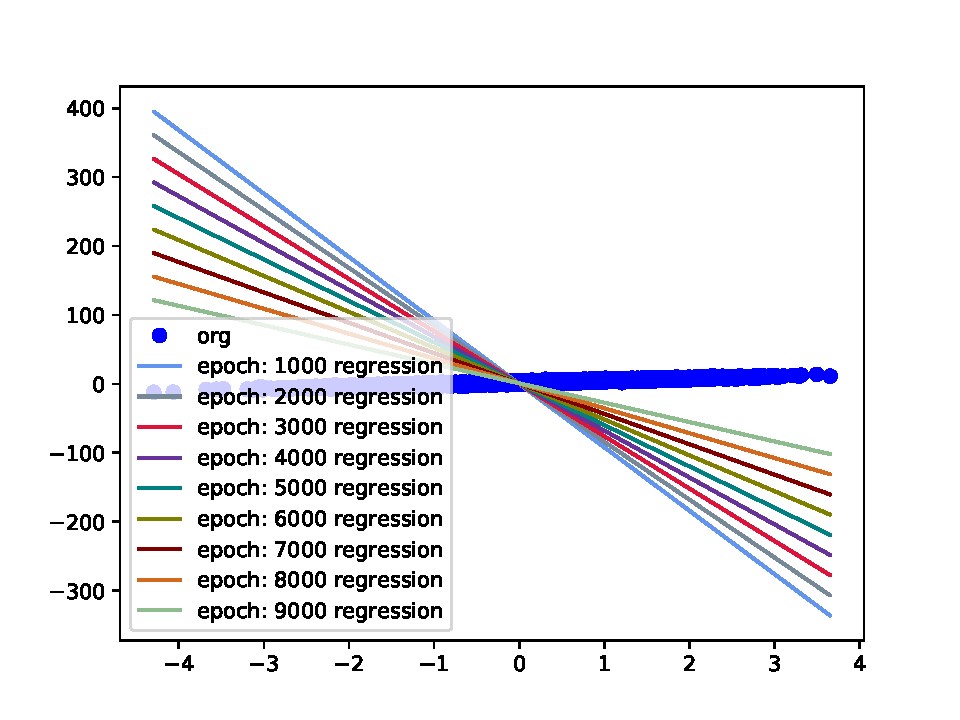
\includegraphics[scale=0.5]{imgs/epoch.pdf}
  \caption{Training duration with a large initiail parameter}
  \label{epoch}
\end{figure}

\subsection{Noise in data}
Before this section, I generated noise in data using normal distribution. Table \ref{noise} shows the results of different noise distribution. The distribution of noise can affect the prediction. Table \ref{normal1} shows the results of normal distribution with different mean. Table \ref{normal2} shows the results of normal distribution with different std. The level of noise is higher, the model is harder to converge.

\begin{table}
  \caption{The performance of different noise in data}
  \label{noise}
  \centering
  \begin{tabular}{lll}
    \toprule
    Noise distribution     & W     & b  \\
    \midrule
    normal(mean=0.0, stddev=1.0)     & 2.9794447 & 1.9967409    \\
    gamma(alpha=1)    & 2.98501      & 2.8410964  \\
    uniform(minval=0)    &2.9989622  &2.502729\\
    \bottomrule
  \end{tabular}
\end{table}

\begin{table}
  \caption{The performance of normal distribution with different mean}
  \label{normal1}
  \centering
  \begin{tabular}{lll}
    \toprule
    mean    & W     & b  \\
    \midrule
    0.0     & 2.9794447 & 1.9967409    \\
    1.0    & 2.964156 & 2.990973  \\
    2.0    &2.9483728 &3.9745786\\
    3.0    &2.924222 &4.9402742\\
    \bottomrule
  \end{tabular}
\end{table}

\begin{table}
  \caption{The performance of normal distribution with different std}
  \label{normal2}
  \centering
  \begin{tabular}{lll}
    \toprule
    mean    & W     & b  \\
    \midrule
    1.0    & 2.9794447 & 1.9967409 \\
    2.0    &2.8706882 &1.9283952\\
    3.0    &2.6891909 &1.8024324\\
    \bottomrule
  \end{tabular}
\end{table}

\subsection{Noise in data during training}
First, I tested adding noises(normal distribution: $mean = 0.$, $stddev=1.$) in data per epoch. The predicted parameters are $W = 1.4970689$, $1.8999192$.Then, I added noises(normal distribution: $mean = 0.1$, $stddev=0.1$) in weights per epoch. The predicted parameters are $W = -15.267623$, $1.1710013$. Finally, I added noises(normal distribution: $mean = 0.001$, $stddev=0.002$) in learning rate per epoch. The predicted parameters are $W = 2.9953077$, $2.007313$. 

Noise in data and weight will change the performance of the model. If noise in learnign rate is reseanable, it may affect training time. But it will not change the general performance of the model, except it reaches local minima. For example, it may lead to faster convergence or make the model hard to coverge. 

On other classification problems and mathematical models, noise in data and weight will definetly reduce model's performance. But adding small noise in learning rate may make it possible to get rid of local minima.  

\subsection{Significance of seed}
If I use the same seed to generate noise, I will get the same results every time I run the code without change any parameters. Because the pseudorandom number generating algorithms is designed to performing operation on a seed. So the result of algorithms is determined by the seed. If I want to change the result every time, I can use current time as the seed.

\subsection{Dropout}
On real world dataset, I'll try to dropout some values because usually the outliers are not 

\subsection{GPU VS CPU}

\section{Problem 2}

\end{document}
